% !TeX root = ../main.tex

\chapter{引言}

\section{研究背景与意义}
% 推荐系统很重要
推荐系统是基于用户的兴趣爱好,从海量候选集中帮助用户找到感兴趣的内容\cite{li2020collaborative, dhelim2020personality}。推荐系统的应用场景非常广泛,包括社交推荐\cite{li2014social, tang2013social}、商品推荐(电商)\cite{zhang2012research, wu2008clustering}、长短视频推荐\cite{davidson2010youtube, hongliang2015video}和新闻推荐\cite{li2011scene, zihayat2019utility}等等。从商业价值角度来看,推荐系统具有极高的商业价值,如图~\ref{fig:apps}所示,大量应用使用到推荐系统。例如阿里巴巴旗下的电商平台淘宝\cite{gong2020edgerec}、快手短视频\cite{cai2023reinforcing}、字节跳动旗下的抖音短视频、腾讯旗下以社交平台微信为核心的众多业务平台等等。

\begin{figure}
  \centering
  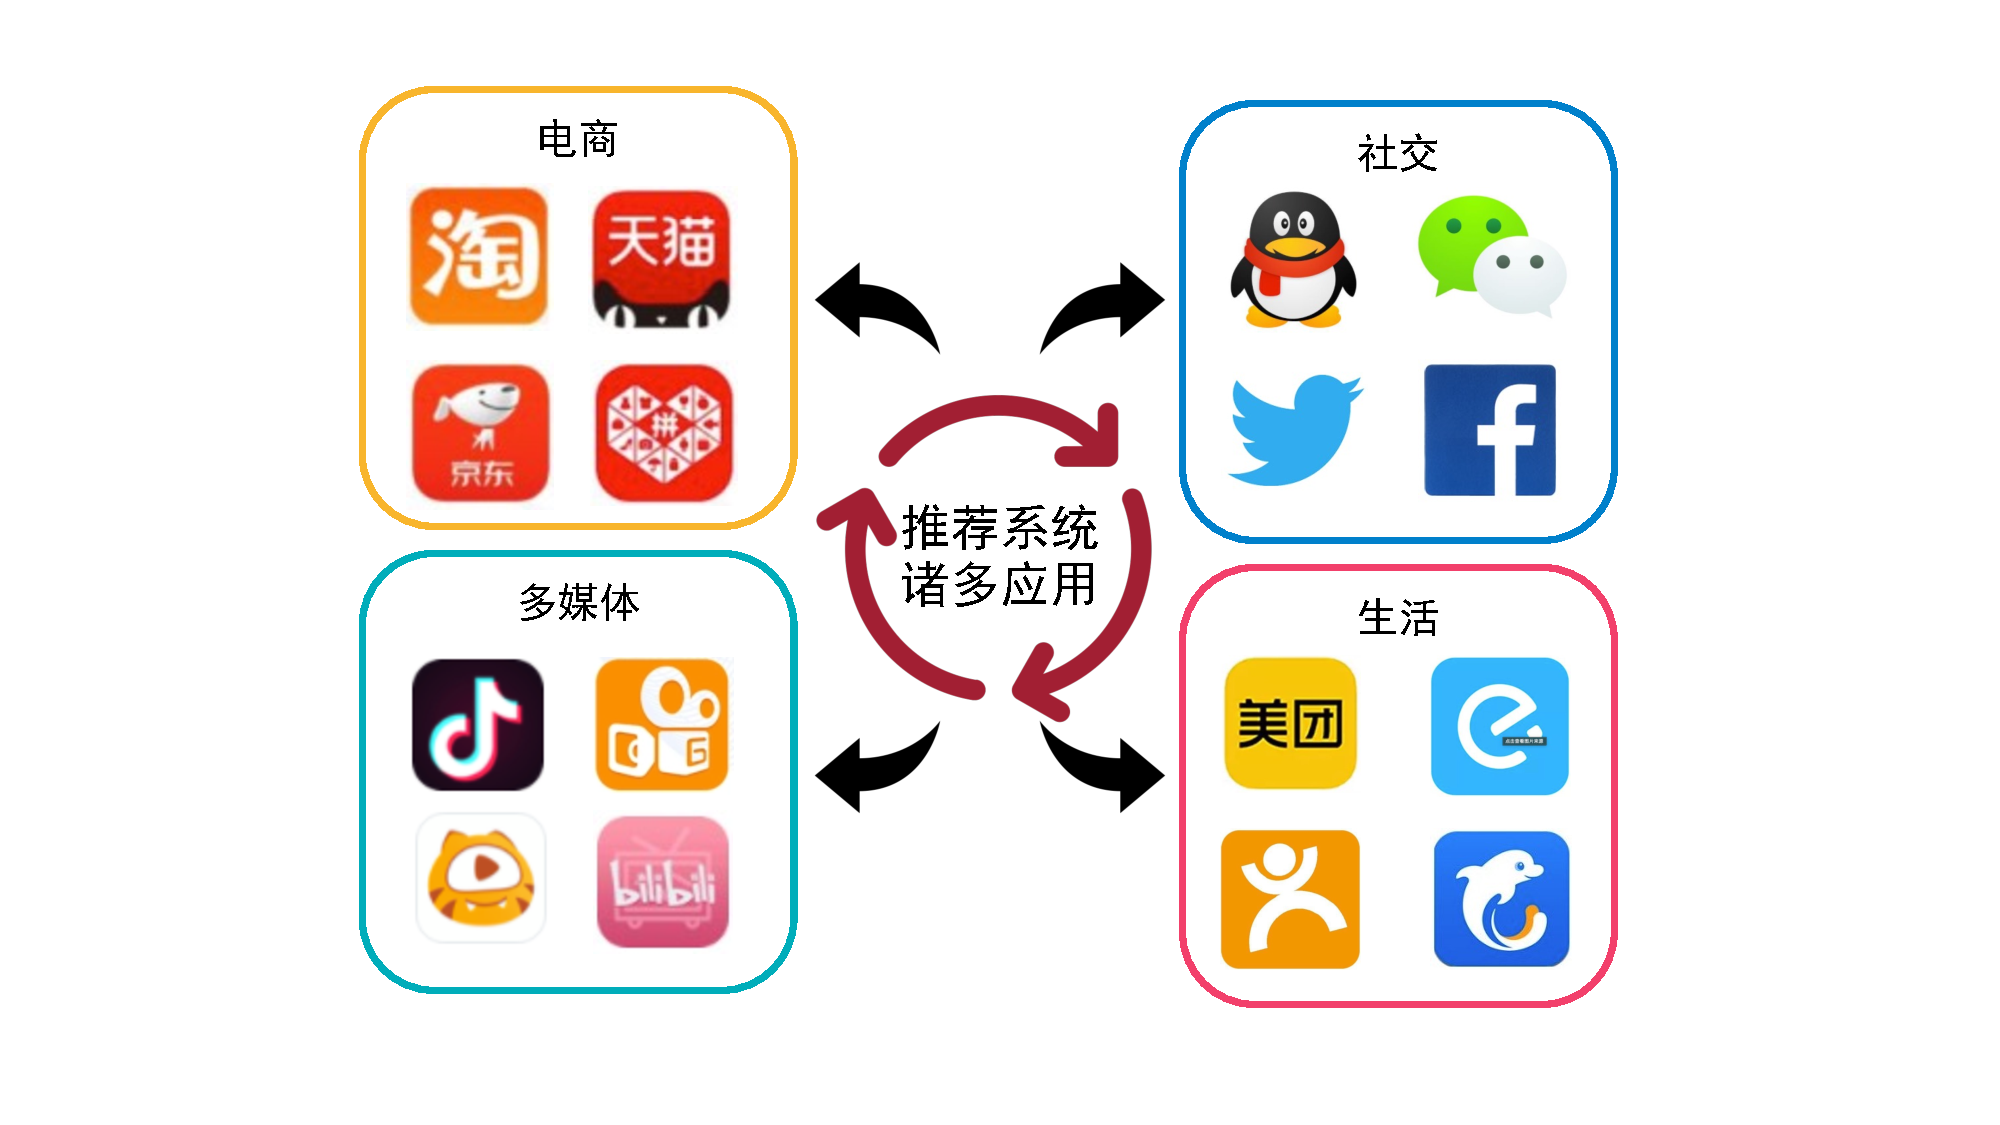
\includegraphics[width=0.6\linewidth]{figures/Introduction/apps.pdf}
  \caption{推荐系统的大量应用场景}
  \label{fig:apps}
\end{figure}

% 推荐系统的流程
随着深度神经网络技术的发展,向量化的推荐算法成为实际场景中广泛使用的算法\cite{su2020link, dhaware2020tourism, mukhopadhyay2008product}。向量化推荐系统将用户和物品编码成向量,在推荐过程中主要包括召回阶段和排序两大阶段,如图~\ref{fig:flowchart}所示。其中召回阶段负责从海量的数据中(百万-亿)初筛出一小部分数据(几十-百)用于后续的个性化推荐。排序阶段就是在召回阶段所筛选出数据的基础上,额外考虑用户的个性化信息,例如历史行为、用户画像等。最终将若干个结果推荐给用户。

\begin{figure}
  \centering
  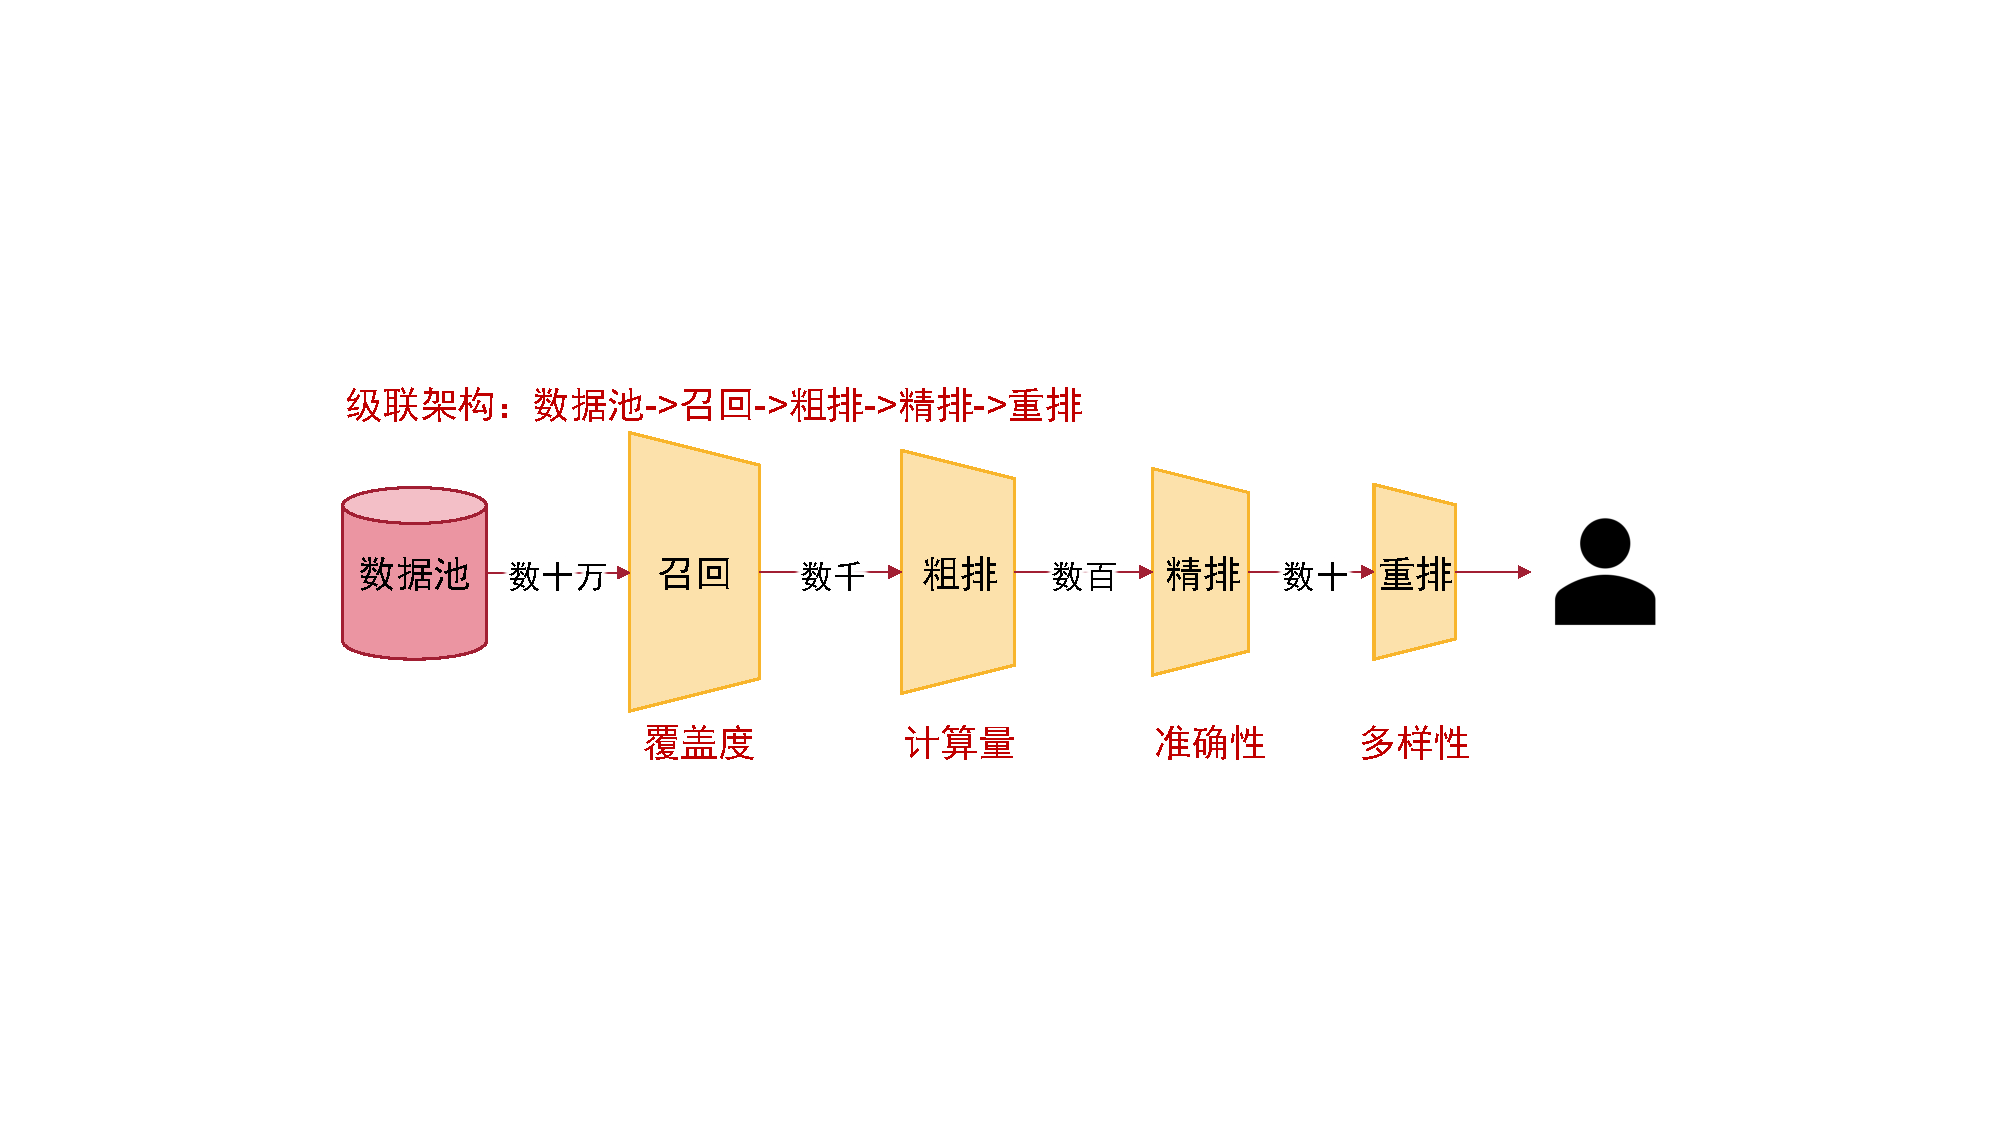
\includegraphics[width=0.9\linewidth]{figures/Introduction/flowchart.pdf}
  \caption{一般推荐系统流程图}
  \label{fig:flowchart}
\end{figure}

% 近似近邻搜索是推荐系统的核心组件
随着大数据时代的到来,近似近邻搜索成为推荐系统的核心组件\cite{chen2022approximate}。原因是推荐系统所需要处理的数据规模急剧增加,近似近邻搜索算法相比其他算法可以更快的完成对于大规模数据的高效处理\cite{wang2021comprehensive, jiang2020clustering, xu2022proximity}。如何进一步加速近似近邻搜索成为我们必须要面对和解决的问题。

% 基于图的近似近邻搜索目前被广泛使用由于其优越的性能
基于图的近似近邻搜索算法由于其优越的性能而被广泛使用\cite{chen2022finger, yu2022gpu, groh2022ggnn}。该算法将待搜索的向量看做高维空间中的点,通过一定的规则在这些点之间连接边,最后形成一张图。在线搜索的过程中,根据用户编码得到的查询向量,在图上进行搜索。
% 算法一般包括构建算法和搜索算法。构建算法就是在给定待搜索的数据集上构建图索引,搜索算法就是在图索引上根据给定的查询搜索与其最相似的结果。

% 基于图的近似近邻搜索存在构建和搜索方面的问题
随着大数据时代的到来,基于图的近似近邻搜索面临以下问题导致其性能难以支持海量数据下的推荐系统。首先,基于图的近似近邻搜索相比其他类型的算法需要更长的构建时间,随着新增数据量的增加,该方法面临严重的问题,可能导致图索引上的数据并不是最新,无法给用户准确的推荐物品。其次,现有硬件架构的低效导致基于图的近似近邻搜索在大规模数据的情况下,在推荐系统实时性的约束下,无法达到业务所需要的吞吐率。最后,现有基于图的近似近邻搜索的分布式算法的拓展性很差,考虑到单机的资源总是有限的,现有分布式算法的低效限制了其处理更大规模数据的潜力。

\section{研究现状}

近邻搜索(Nearest Neighbor Search,NNS)是在给定集合中找到与给定点最接近(或最相似)的点的优化问题\cite{nns-wiki}。精确求解这一问题只能采用暴力检索的方式,在大规模问题中难以应用。因此,研究者转向近似近邻搜索(Approximate Nearest Neighbor Search,ANNS),通过一定程度下可接受的精度损失,换取检索时间的极大降低。近似近邻搜索的核心思想就是将数据在某个维度的空间中做切分,减少需要遍历的数据量。根据空间划分方式的不同,大致可以分为以下四类:基于量化\cite{pq-2010, opq-2013, douze2016polysemous, zhang2019grip, kalantidis2014locally, abdelhadi2019accelerated}、基于树结构\cite{kdtree-2008, Annoy, houle2014rank,arora2018hd, muja2014scalable, wang2013trinary}、基于哈希(Locality-sensitive Hashing,LSH)\cite{lsh-1999, lsh-2004, sh-2008, sun2014srs, terasawa2007spherical, liu2014sk}和基于图结构\cite{kgraph-2011, nsw-2014, hnsw-2018, nsg-2019, dpg-2019}方法。如图~\ref{fig:ganns-vs-other}所示,由于实际数据的维度灾难等问题,基于图结构的近似近邻搜索方法取得了优于其余方法的效果,因此成为近年来的研究热点。本节将重点介绍基于图的近似近邻搜索方法的研究现状,同时也会对其余类型的方法做简要介绍。

\begin{figure}
  \centering
  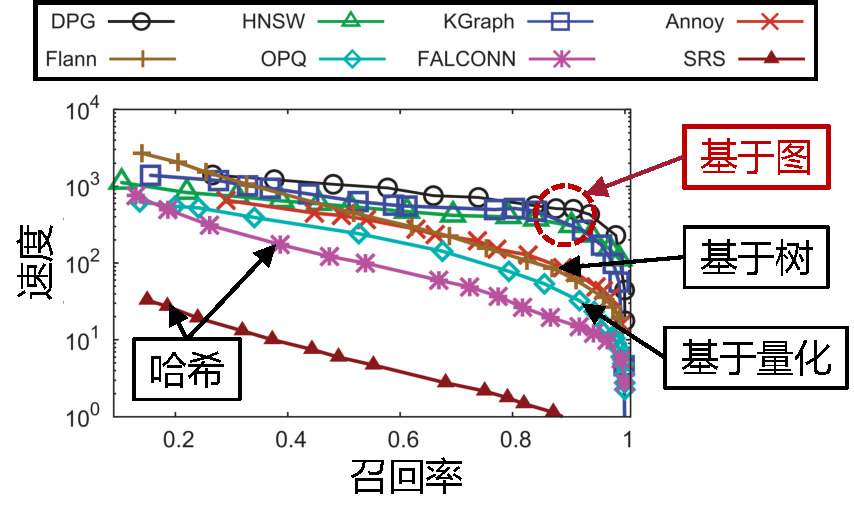
\includegraphics[width=0.7\linewidth]{figures/Introduction/ganns-vs-other.pdf}
  \caption{不同类型的近似近邻搜索方法的比较\cite{dpg-2019}(右上更好)}
  \label{fig:ganns-vs-other}
\end{figure}


\subsection{非图的近似近邻搜索方法}
非图的近似近邻搜索方法在构建开销和索引开销方面相比图方法具有一定的优势,因此在某些小数据集、存储资源匮乏的场景下也会被使用。非图的近似近邻搜索方法主要包括以下三类:
\begin{itemize}
  \item 基于量化的近似近邻搜索。这种方法通过量化编码的方式来近似表示原始数据空间。量化编码的好处一方面可以降低计算复杂度,另一方面也可以降低数据存储开销,但是量化会引入一定的近似导致最终搜索结果的准确性不足。
  其中的代表性方法包括:乘积量化\cite{pq-2010}(Product Quantization,PQ)是最具代表性的方法,它将数据在维度上切分为若干个子空间,然后使用每个子空间内的聚类中心点作为该类的编码。计算时只需要计算查询和这些编码的距离,将向量距离计算转换为查表操作。优化乘积量化\cite{opq-2013}(Optimized Product Quantization,OPQ)是在乘积量化的基础上,通过预处理的方式降低量化引入的误差。

  \item 基于树的近似近邻搜索。这种方法通过树结构的方式对数据空间进行划分,进而实现减少搜索时计算量的目的。该方法一般用于数据维度较低的场景中,一旦数据维度变高,该类方法的搜索效率将会显著降低\cite{AQA-1998}。
  其中代表性方法包括:K-D树\cite{kdtree-2008}(K-Dimensional Tree),K-D树通过所有的非叶子结点将数据空间逐级切分,每个叶子结点都代表一个多维数据。Annoy\cite{Annoy}(Approximate Nearest Neighbors Oh Yeah)以垂直平分两个聚类中心点连线的超平面将数据空间切分,然后通过递归的方式减少空间中的数据数量。

  \item 基于哈希的近似近邻搜索。这种方法是通过设计哈希函数将原始数据映射为哈希数据,进而降低计算的复杂度,同时还可以起到压缩数据的作用,但是哈希函数不可避免的会导致数据的信息损失进而影响精度。
  其中的代表性方法包括:局部敏感哈希\cite{lsh-1999,lsh-2004}(Locality-Sensitive Hashing,LSH)的核心思想是数据之间越相似,那么它们产生哈希冲突的概率也就越高。因此通过哈希函数后落入同一个哈希桶内的数据之间的相似概率更高,但是该方法还存在负载不均衡等问题。谱哈希\cite{sh-2008}(Spectral Hashing,SH)相比局部敏感哈希利用了数据空间的分布特性,可以从数据中学习哈希函数实现更优的映射。
\end{itemize}


\subsection{\ganns}
\ganns 方法将有限集合中的向量映射成高维空间中的点,核心思想是通过点之间的连接关系减少待搜索的空间。在构建阶段,通过一定的规则在这些点之间建立连接,这些点和边所组成的结构我们称之为图索引。在搜索阶段,对于用户给定的查询,在图上检索与查询最相似的若干个结果。我们从图索引上的某个点(搜索起始点)开始,迭代地搜索沿着这些边更接近查询的点。构建过程是连接这些点之间的边。不同的\ganns 方法之间的主要区别在于构建过程中使用的算法。

% TODO总结一下核心思想
\citet{hnsw-2018}等人提出的分层导航小世界图(Hierarchical Navigable Small World graphs, HNSW)是一种典型的\ganns 方法。相比之前的导航小世界图\cite{nsw-2014}(Navigable Small World graph,NSW)方法主要有两方面的改进,首先是层次化,HNSW由多个NSW图层组成;其次是选边策略,HNSW采用的是基于相对邻域图\cite{rng-1980}(Relative Neighbourhood Graph,RNG)的策略,该策略可以筛选出更加分布更加离散的邻居分布。在构建过程中,基向量中的每个点逐个添加到图索引中。每个点所在的最高层由一个概率指数衰减的随机函数决定,然后这个点需要添加到最高处以下的所有层中。然后,最底层包含数据空间中的所有点。

% TODO:Check 括号格式
\citet{nsg-2019}等人提出了导航扩展图(Navigating Spreading-out Graph,NSG),为预先构建的\textit{k-}近邻图(\textit{k-}Nearest Neighbor Graph,\textit{k-}NNG)上的每个点重新选择邻居。基于单调相对邻域图(Monotonic Relative Neighborhood Graph,MRNG)\cite{nsg-2019}的邻居选择策略保证每一步都比前一步更接近查询,但会导致过度的构建复杂度。因此,NSG采用近似的MRNG策略,将中心点确定为搜索起始点,减少构建复杂度。但NSG很难实现增量方式的构建,因为它需要预先构建好\textit{k-}近邻图。

多样化邻近图(DPG) \cite{dpg-2019}是在KGraph \cite{kgraph-2011}的基础上进行优化。其方法是对现有的k-近邻($k$-NN)图进行多样化,并添加反向边以提高搜索性能。对于数据点$p$,我们假设在$p$的近邻列表${L_N}$中有两个点$a$和$b$。然后定义角度$\theta (a,b) = \angle apb$。DPG使用贪婪启发式算法从${L_N}$中选择一个子集$S$,以最大化$S$中两点之间的平均夹角。此外,DPG设置图中某个点的最大连通邻居数(即$k$),以找到$k$ NN图的多样性和邻近性之间的良好权衡。

% \subsection{\ganns 的硬件工作}
% diskann spann ggnn


\section{研究内容与主要贡献}

\begin{figure}
  \centering
  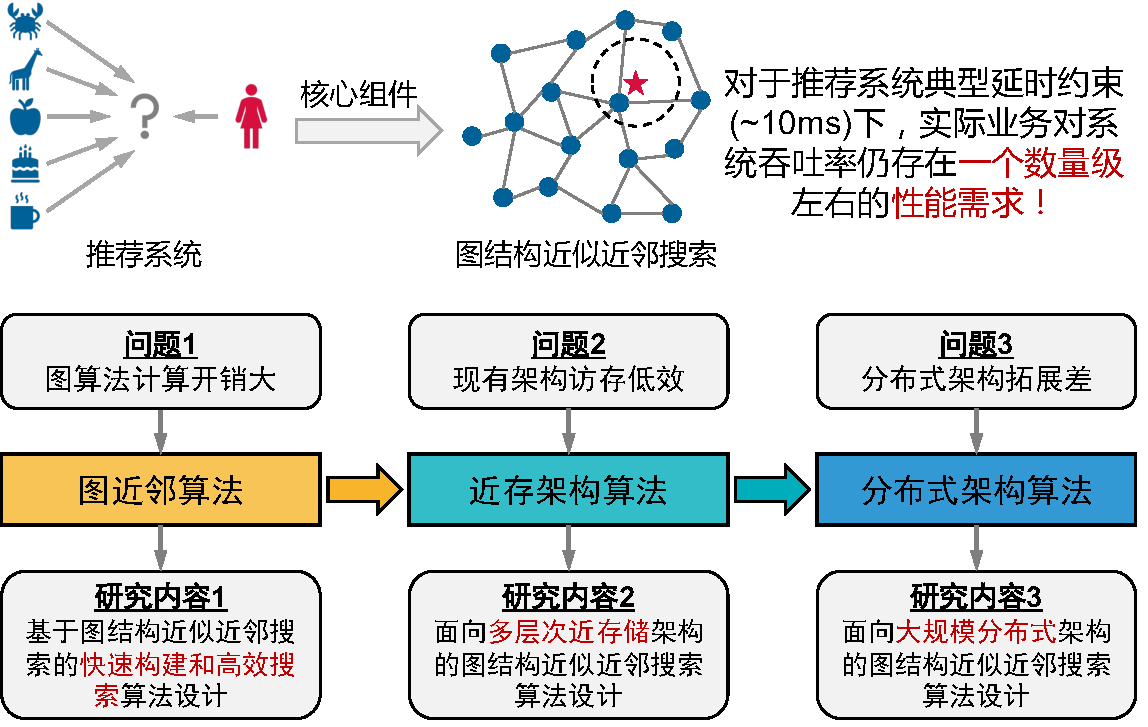
\includegraphics[width=0.7\linewidth]{figures/Introduction/overview.pdf}
  \caption{本文的整体研究内容}
  \label{fig:overview}
\end{figure}

% 数据检索中图方法很好,但是在大数据时代下面临挑战
综上所述,尽管基于图的方法相比其他类型的近似近邻搜索方法在以推荐系统为代表的数据检索问题中表现出更优的性能,但其仍然存在的三个问题限制了在大数据时代下的应用潜力。
首先,\ganns 方法相比其他方法具有更长的构建时间\cite{dpg-2019},其原因是在构建阶段的计算开销大。因此在海量数据下难以做到对新增数据的及时更新,进而影响推荐系统的服务质量。其次,\ganns 方法在现有硬件架构上运行效率低下,其原因是\ganns 在计算过程中涉及大量的数据搬运,进而在冯诺依曼这种存算分离的架构上表现低效。以CPU为例,整个执行过程的80\%以上开销在访存,这一问题在大规模数据下会更为严重。最后,随着数据规模的不断增加,单机的处理能力总是有限的,而现有针对多机的\ganns 方法存在拓展性差的问题。总的来说,\ganns 的这些问题限制了在大数据时代下的应用潜力,以推荐系统这一典型场景为例,仍然存在一个数量级以上的性能差距。

% TODO:替换“我们”这种表述
图~\ref{fig:overview}给出了本文的整体研究内容,本文主要从构建算法、近存算法和多机算法三个方面开展研究设计,分别针对上述问题提出解决方案。其中后两个研究内容主要是针对搜索算法的,因为在实际中搜索算法是在线进行的。
针对第一个问题,本文研究高效的构建算法设计,以降低构建阶段的计算开销。\todo{具体解法是什么?}

针对第二个问题,本文研究面向近存架构的高效算法设计,结合不同层级的近存架构特点设计相应的算法,充分发挥近存架构的潜力。首先本文对\ganns 的搜索算法所设计的算子进行抽象和分析,建立了硬件分析模型。然后基于硬件分析模型,对近内存处理架构提出了并行方案的设计。最后考虑到大规模数据下的情况,拓展了近外存处理架构,并结合外存的访存特点对算法进行了流水设计。

针对第三个问题,本文研究面向多机分布式的高效算法设计,有效提高了\ganns 方法的拓展性。首先本文在现有多机方法的基础上提出了一套通用的多机并行框架,并分析了现有无通信方式在图结构下的不足和问题。然后针对多机并行框架具有更高理论上限的全图方式,在直接的方案下会严重受限于通信开销这一问题,分别提出了索引预先加载策略和特征延迟处理策略,大幅减少了通信开销,有效提升了\ganns 方法在大规模数据下的拓展性。

% \begin{figure}
%   \centering
%   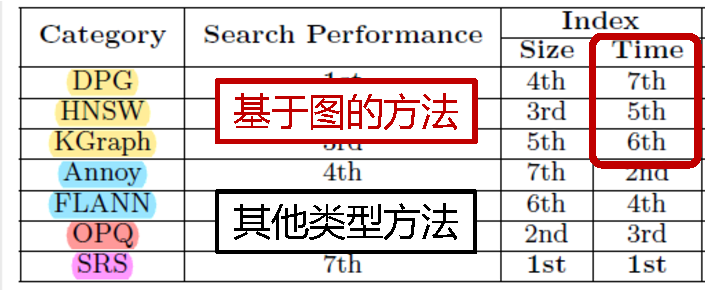
\includegraphics[width=0.6\linewidth]{figures/Introduction/ganns-index.pdf}
%   \caption{基于图的近似近邻搜索方法需要更长的构建时间\cite{dpg-2019}}
%   \label{fig:ganns-index}
% \end{figure}



\section{本文的组织结构}
本文的组织结构如下:

首先,本文在第1章中详细阐述了本文的研究背景和意义,并介绍了相关工作的研究现状,指出\ganns 方法所面临的问题和优化机会,并在最后简要总结了本文的主要贡献和研究内容。

第2章介绍相关研究的基础知识。首先介绍了\ganns 的问题定义、构建过程和搜索过程,然后介绍了近存架构的概述。

第3章针对\ganns 中构建阶段的计算开销大的问题,研究构建算法的设计。\todo{内容}

第4章和第5章重点考虑\ganns 的搜索阶段的加速。第4章针对\ganns 在现有硬件架构上面临执行能效低下的问题,研究高效的近存算法设计。

第5章针对\ganns 拓展性差,难以处理更大规模数据的问题,研究高效的多机算法设计。

最后,第6章总结了本文的核心思路和主要创新点。并提出了本文工作在未来可能的研究方向。